% !TeX root = ../main.tex
\section{Cohomology} % (fold)
\label{sec:cohomology}

A \textbf{cochain complex} is a sequence $\tilde{\C} = (C^*, \delta_*)$ of $\R$-modules $C^k$ consisting of \textbf{cochains} and module homomorphisms known as \textbf{coboundary maps} $\delta_k:C^k\to C^{k+1}$.
As in homology we have the property that $\delta_{k+1}\circ\delta_k = 0$ for all $k$, leading to a familiar definition of the \textbf{cohomology} of $\tilde{\C}$
\[ H^k(\C) = \ker\delta_k/\im\delta_{k-1}.\]
The equivalence classes of $H^k(\C)$ consist of \textbf{$k$-cocycles}: elements of $\ker\delta_k$ that differ by a \textbf{$k$-coboundary} in $\im\partial_{k-1}$.
Such cocycles are said to be \textbf{cohomologous} if they belong to the same equivalence class in $H^k(\C)$.

The simplest construction of a cochain complex is to dualize a chain complex.
For a chain complex $(C_*,\partial_*)$ define $C^k$ to be the module of homomorphisms $\psi:C_k\to\R$.
The coboundary maps $\delta_k$ are defined for cochains $\psi:C_k\to\R$ and $k$-simplices $\sigma\in K$ as
\[\delta_k\psi(\sigma) = \psi(\partial_k\sigma).\]
It is in this sense that the cohomology $H^k(\tilde{\C})$ of a cochain complex $\tilde{\C}$ constructed from a chain complex $\C$ is the algebraic dual of the homology $H_k(\C)$ of $\C$.
Moreover, the \textbf{Universal Coefficient Theorem} implies that, for finite dimensional homology groups, there is an isomorphism between homology and cohomology groups.
It follows that there is an isomorphism between the persistent homology and \textbf{persistent cohomology} of a filtration $\K$.

While simplicial homology identifies equivalence classes of cycles in a chain complex simplicial cohomology instead identifies equivalence classes of homomorphisms from the chain complex to a field.
In essence, homology and cohomology offer different perspectives that reveal the same structure, homology rooted in geometry and cohomology in algebra.
As we will see the language of cohomology offers a more robust setting for using the algebraic structure of cocycles.

\subsection{Representative Cycles and Cocycles}

Let $K = \rips^\alpha(P)$ be the rips complex of a finite metric space $P$.
We can find a basis for each homology group $H_p(K)$ and cohomology group $H^p(K)$ consisting of $p$-cycles and $p$-cocycles, respectively.
In general, $p$-cycles represent $p$-dimensional holes in the simplicial complex $K$, where $p$-cocycles can be understood as ``blocking chains.''

\begin{figure}[htbp]
\centering
    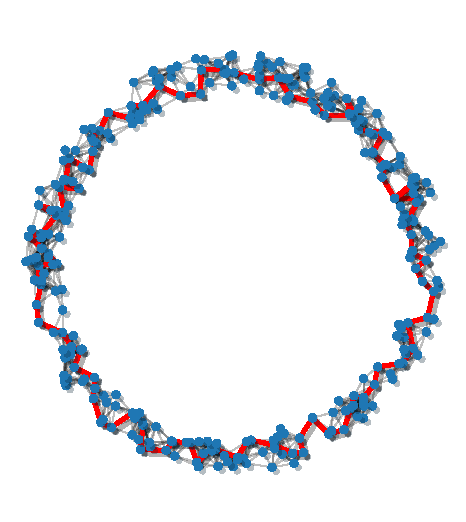
\includegraphics[scale=1.]{figures/homology_cycle.pdf}
    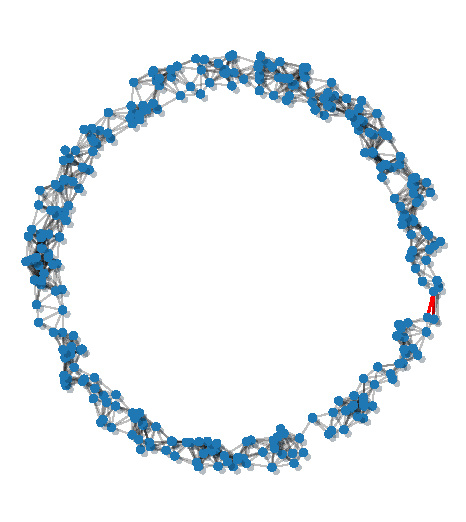
\includegraphics[scale=1.]{figures/cohomology_cocycle.pdf}
    % 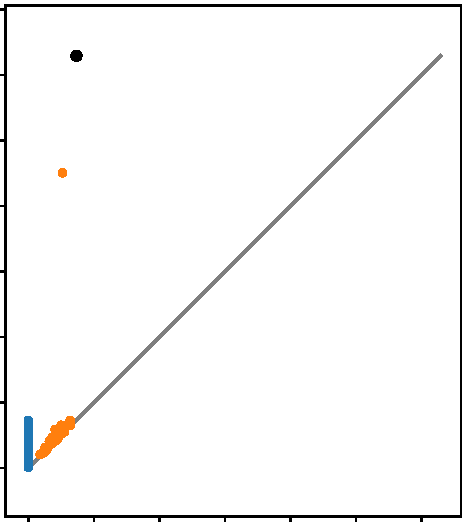
\includegraphics[scale=0.66]{figures/circular_dgm1.pdf}
    \caption{Consider a noisy sample $X$ of the 1-sphere, or circle, $\mathbb{S}^1$ with radius 1.
            Let $K = \rips^\e(X)$ for $\e\approx 0.14$, 1-skeleton shown.
            (Left) In red, the edges of a representative cycle of $H_1(K)$.
            (Right) In red, the edges of a representative cocycle of $H^1(K)$.
            Note that while the representative cycle clearly identifies equivalence class of 1-cycles of $X$, all paths around the circle, the representative cocycle represents the class of ``blocking'' cochains.}
    \label{fig:cycles}
\end{figure}

\subsection{Circular Coordinates}

Cocycles are particularily useful in distributing the information contained in each cohomology basis element throughout a simplicial complex.
This is one application of the theory of discrete exterior calculus, which we will illustrate with an algorithm presented by de Silva et al.~\cite{desilva09persistent}.
The work uses representative cocycles of features in persistent cohomology to construct a circle-valued function on the vertex set referred to as \textbf{circular coordinates}.
The distinction is made with classical cartesian coordinates which are often viewed as values on a line (an axis).

\begin{figure}[htbp]
\centering
  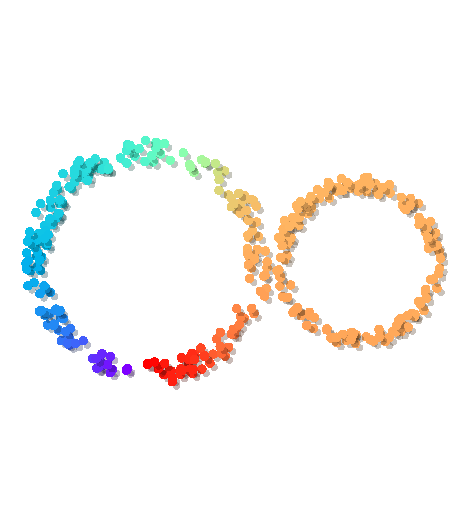
\includegraphics[scale=0.8]{figures/circular_coords1.pdf}
  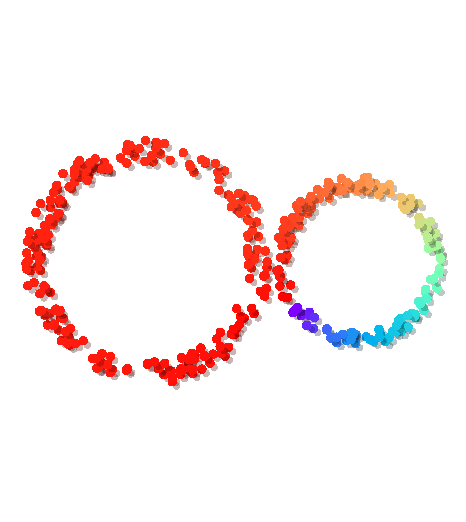
\includegraphics[scale=0.8]{figures/circular_coords2.pdf}\\\vspace{-7ex}
  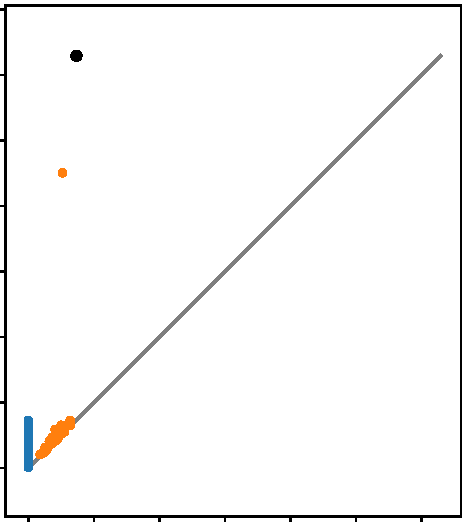
\includegraphics[scale=0.5]{figures/circular_dgm1.pdf}\hspace{1.3in}
  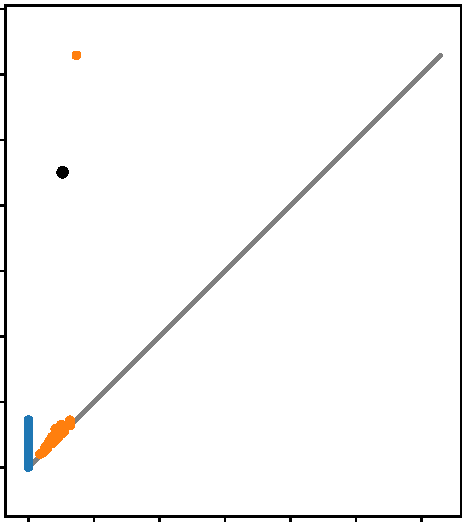
\includegraphics[scale=0.5]{figures/circular_dgm2.pdf}
   \caption{(Top) Circular coordinates as colorings on a set of points $P$ sampled from two noisy circles with radii 1 and 0.7.
        The two coordinates were constructed from representative 1-cocycles corresponding to persistent features in the persistent cohomology of the rips complex of $P$ (bottom).
        Note that each representative cocycle yeilds coordinates which are localized to the corresponding feature.}
   \label{fig:circular}
\end{figure}

Let $K$ be a simplicial complex constructed over a point cloud $P$ at some scale $\e_{max}$.
The algorithm first computes the persistent cohomology of $K$ over a prime field $\F_p$ for prime $p > 2$.
Any point $(b, d)$ in the 1-dimensional persistence diagram corresponds to a representative cocycle $\alpha_p\in C^1(K;\F_p)$.
Let $K^\e$ be the subcomplex of $K$ for some $\e\leq \e_{max}$ in the interval $[b, d]$ and $\alpha^\e_p\in C^1(K^\e;\F_p)$ be the restriction of $\alpha_p$ to simplices in $K^\e$.
For our calculations we chose the midpoint $\e = \frac{b+d}{2}$.
Moving forward let $K = K^\e$ and $\alpha_p = \alpha^\e_p$.

Next, ``lift'' the cocycle $\alpha_p$ over a prime field to an integer cocycle $\alpha\in C^1(K;\Z)$ which reduces to $\alpha_p$ modulo $p$.
In practice we can almost always construct $\alpha$ by taking the coefficients of $\alpha_p$ in $\F_p$ and replacing them with integers in the correct congruence class modulo $p$, preferring coefficients close to zero in the range
\[ \{-(p-1)/2,\ldots,-1,0,1,\ldots,(p-1)/2\}. \]
There are some edge cases in which the boundary $\delta_1\alpha\neq 0$, in which case $\alpha$ is not a valid integer cocycle, however for the sake of brevity we will assume that $\delta_1\alpha = 0$.

Noting that any integer cocycle $\alpha\in C^1(K;\Z)$ is also a real cocycle in $C^1(K;\R)$ we would now like to find the ``smoothest'' real cocycle $\overline{\alpha}\in C^1(K;\R)$ that is cohomologous to $\alpha$.
Such a cocycle is known as a \textbf{harmonic cocycle} representing the cohomology class $[\alpha]$.
Each of the spaces $C^i(X;\R)$ comes with a natural Euclidean metric: for $f\in C^0(K;\R)$, $\alpha\in C^1(K;\R)$ %, and $A\in C^2(K;\R)$
\begin{align*}
    \|f\|^2 = \sum_{p\in K^0} |f(p)|^2\\
    \|\alpha\|^2 = \sum_{e\in K^1} |\alpha(e)|^2 % \\
    % \|A\|^2 = \sum_{t\in K^2} |A(t)|^2
\end{align*}
where $K^k$ denotes the collection of $k$-simplices in $K$.
A circle-valued function $\theta$ is said to be ``smooth'' if its total variation across the edges of $K$ is small.
The variation of $\overline{\alpha}$ across edges $e\in K^1$ is captured by the terms $|\overline{\alpha}(e)|^2$, so we seek to minimize $\|\overline{\alpha}\|^2$.

\begin{proposition}
    Let $\alpha\in C^1(K; \R)$.
    There is a unique solution $\overline{\alpha}$ to the least-squares minimization problem
    \[ \argmin_{\overline{\alpha}} \{\|\overline{\alpha}\|^2\mid \exists f\in C^0(K;\R),\ \overline{\alpha} = \alpha + \delta_0 f\}.\]
    Moreover, $\overline{\alpha}$ is characterized by the equation $\delta_0^*\overline{\alpha} = 0$, where $\delta_0^*$ is the adjoint of $\delta_0$ with respect to the inner products on $C^0, C^1$.
\end{proposition}

We can integrate the resulting harmonic cocycle $\overline{\alpha}$ to obtain a circle-valued function $\theta$ on the vertex set $X^0$ as follows.
If $K$ is connected (if not, each connected component can be treated separately) select a starting vertex $x_0$ and set $\theta(x_0) = 0$.
Then find the shortest path from $x_0$ to each remaining vertex - when a new vertex $b$ enters the structure via an edge $e$ from vertex $a$ to $b$ assign $\theta(b) = \theta(a) + \overline{\alpha}(e)$.

% \vspace{0.25in}
% \textbf{TODO} Cochains as functions on simplicial complexes
% \vspace{0.25in}

% \subsection{Discrete Exterior Calculus}

 % and $\K = \{K_i\}_{i=1,\ldots,n}$ be a filtration of simplicial complexes $K_i = \rips^\alpha_i(P)$ for $\alpha_1 < \alpha_2 <\ldots < \alpha_{n-1} < \alpha_n = \alpha$.
 % While this does not have an immediate application to our investigation of coverage in homological sensor network it is a powerful tool which may be used for future research in coordinate free sensor networks.

% section cohomology (end)
